\documentclass{article}
% \usepackage[utf8]{inputenc}. % default style
\usepackage{hyperref, graphicx, floatrow, tikz} % adds linking on the doc
\usetikzlibrary{chains,mindmap,tree,shapes,arrows}

\usepackage{titlesec}

\setcounter{secnumdepth}{4} % use \paragraph{} for sub sub sub section


\setlength\parindent{15pt}           % wider style with less white space 
\addtolength{\oddsidemargin}{-.875in} % using this for now bc I like wider and the white space way is having issues
\addtolength{\evensidemargin}{-.875in}
\addtolength{\textwidth}{1.75in}
\addtolength{\topmargin}{-.875in}
\addtolength{\textheight}{1.75in}

   %%%% Packages

\usepackage{amssymb}
\usepackage{amsfonts}
\usepackage{amsmath}
\usepackage{amsthm}

\usepackage{savesym}
\usepackage{bm}
\usepackage{algorithm}
\usepackage{algorithmic}
\floatname{algorithm}{Procedure}
\renewcommand{\algorithmicrequire}{\textbf{Input:}}
\renewcommand{\algorithmicensure}{\textbf{Output:}}

\savesymbol{comment}
\usepackage{easyReview}

\usepackage{comment}  %% block comments

\usepackage{color}
\newcommand{\vnote}[1]{\textcolor{red}{Vinod's note: {#1}}}
\newcommand{\leonote}[1]{\textcolor{red}{Leo's note: {#1}}}
\newcommand{\writeme}{\textcolor{red}{Write Me}}

\newcommand{\round}[1]{\lceil #1 \rfloor}
\newcommand{\floor}[1]{\lfloor #1 \rfloor}
\newcommand{\bigfloor}[1]{\big\lfloor #1 \big\rfloor}
\newcommand{\Bigfloor}[1]{\Big\lfloor #1 \Big\rfloor}

\newcommand{\anglebracks}[1]{\langle #1 \rangle}

\makeatletter
\newcommand\newtag[2]{#1\def\@currentlabel{#1}\label{#2}}
\makeatother

%
% defining the \BibTeX command - from Oren Patashnik's original BibTeX documentation.
\def\BibTeX{{\rm B\kern-.05em{\sc i\kern-.025em b}\kern-.08emT\kern-.1667em\lower.7ex\hbox{E}\kern-.125emX}}
    
    

\newtheorem{theorem}{Theorem}[section]
\newtheorem{definition}{Definition}[section]
\newtheorem{corollary}{Corollary}[theorem]
\newtheorem{lemma}[theorem]{Lemma}
\newtheorem{remark}{Remark}[section]

\newcommand{\calA}{\mathcal{A}}
   
   \newcommand{\olea}{\alpha}
    \newcommand{\oleb}{\beta}
    \newcommand{\olex}{x}
    \newcommand{\oleg}{\gamma}
    \newcommand{\veca}{\boldsymbol{\olea}}
    \newcommand{\vecb}{\boldsymbol{\oleb}}
    \newcommand{\vecx}{\mathbf{\olex}}
    \newcommand{\vecg}{\boldsymbol{\oleg}}
    
    \newcommand{\encd}[1]{[\![ #1 ]\!]}
    
    \newcommand{\getsr}{\xleftarrow{\$}}
    
    \newcommand{\ring}{\mathcal{R}}
    \newcommand{\Z}{\mathbb{Z}}
    \newcommand{\olering}{\Z_p}
    
    \newcommand{\KeyGen}{\mathsf{KeyGen}}
    \newcommand{\Encrypt}{\mathsf{Encrypt}}
    \newcommand{\Decrypt}{\mathsf{Decrypt}}
    
    \newcommand{\sk}{\mathsf{sk}}
    \newcommand{\pk}{\mathsf{pk}}
    \newcommand{\evk}{\mathsf{evk}}
    \newcommand{\ct}{\mathsf{ct}}
    
    \newcommand{\Eval}{\mathsf{Eval}}
    \newcommand{\EvalAdd}{\mathsf{EvalAdd}}
    \newcommand{\EvalAddPlain}{\mathsf{EvalAddPlain}}
    \newcommand{\EvalMultPlain}{\mathsf{EvalMultPlain}}
    
    \newcommand{\Sim}{\mathsf{Sim}}
    \newcommand{\Dis}{\mathcal{D}}
    \newcommand{\View}{\mathsf{View}}
    
    \newcommand{\RLWE}{\mathsf{RLWE}}
    
    \newcommand{\Hybrid}{\mathsf{Hybrid}}
    
    \newcommand{\VOLE}{\mathsf{VOLE}}
    \newcommand{\BOLE}{\mathsf{BOLE}}
    
    \newcounter{protocol}
    \makeatletter
    \newenvironment{protocol}[1][htb]{%
        \let\c@algorithm\c@protocol
        \renewcommand{\ALG@name}{Protocol}% Update algorithm name
        \begin{algorithm}[#1]%
    }{
        \end{algorithm}
    }
    \makeatother
    
    \newcommand{\sbline}{\\[.5\normalbaselineskip]}% small blank line

% \usepackage[letterpaper, margin=1in]{geometry}   % wider style with more white space
% \setlength{\parskip}{\baselineskip}
% \setlength{\parindent}{0pt}


\title{Snickerdoodle Protocol}

\author{
  Lucas Novak\\
  \texttt{lucas@snickerdoodlelabs.io}
  \and
  Varun Parthasarathy\\
  \texttt{varun@snickerdoodlelabs.io}
}

\begin{document}

\maketitle
\tableofcontents{}
\pagebreak

% \label{section:security}
% \ref{section:security} example of referencing another section

% footnote{Such noise terms are sometimes referred to as ``flooding" terms.} footnote

% to cite
% \cite{abbe2012privacy} %-- remove this from bib later. As long as it's not used we don't have to worry about it showing up

\section{Abstract}

The Snickerdoodle Protocol aims to enable an open, equitable, and consent-driven federated data market in which individuals will 
collect, own, and authorize the use of their own data. Data is most valuable in the aggregate so that 
it can be leveraged to build predictive models; this results in a data market where centralized aggregators hold 
the only economically valuable role. In this structure, individual users who actually generate data are often 
left with little to no benefit from the value of their data. 

As more and more privacy violations and data breaches continue to occur on a larger scale, it has become apparent that the
centralization of data poses a serious threat to both the individual and the community as a whole as it results in a
single point of failure for malicious actors to focus their efforts. Technology companies, like Apple and Google, have
produced software designed to provide more privacy forward data collection through federated learning and multi-party 
computation models optimized to run on hardware devices that these companies produce. However, these solutions are 
neither auditable nor open, and therefore still leave the end user removed from the value they generate. In addition, 
existing decentralized solutions often focus primarily on the sale of aggregated data sets. The protocol described in this 
whitepaper aims to enable the extraction and collection of new data in real time via edge computing techniques leveraging
a permissionless blockchain as an orchestration layer and control plane. 

This protocol will alleviate these concerns by turning user data into an individualized asset that can be leveraged 
without the need for an initial consolidation step. User-controlled localized ”Data Wallets” will provide an easily usable form 
factor to the end user, while a business-oriented ”Insights Service” will provide analytical and visualization services to entities who wish to extract 
intelligence from the data itself. By providing consent-driven ownership and granular access control to the end-user, we allow them to gain greater sovereignty over their 
digital identity, while freeing businesses from the overhead of regulatory compliance with regard to user data. Our solution will be 
permissionless, community-governed, and self-sovereign, and will provide an alternative to the data economy of today. Internet users 
are already recognizing the need for decentralization in the information economy, as demonstrated by the fact that the Web3 user base 
is growing at a rate comparable to the internet in the 1990s. By properly incentivizing these users, allowing businesses to reach more 
users with less risk, and creating an open protocol for decentralized infrastructure providers, the protocol will facilitate 
a data economy that benefits all. 
\section{Introduction}

The design, implementation, and stability analysis of cryptoeconomic primitives \cite{horne2018crypto} has been an intensive area of research since the emergence of smart contract networks like Ethereum \cite{buterin2014next}. Some prominent examples include Proof of Stake \cite{quantum2011bitcoin} (now the consensus mechanism securing Ethereum itself), tokenization (particularly stable coins backed by digital or traditional assets), curve bonding \cite{graphBondingCurve}, token curated registries \cite{Goldin2018TCR} (TCRs), yield staking, and distributed autonomous organizations \cite{merkle2016daos} (DAOs). 

In short, a cryptoeconomic primitive is a kind of economic game in which the presence of a programmable token asset (which may or may not have a fixed supply) is a prerequisite for the proper functioning of the game and (initial and ongoing) incentive alignment of the participants so that a stable (quasi)equilibrium of the game or market can be achieved without a centralized operator. The list of cryptoeconomic primitive examples given have sought to solve problems in finance, governance, and information asymmetry. 

This work explores a new primitive, stake for ranking, which aims to serve as the core of a self-governing, content-based recommender system. This can be seen as an addition to the tool kit of curation market primitives which, among other things, seek to provide verifiable information to all parties on equal footing. As will be outlined, the token mechanics of stake for ranking also share similarities both with TCRs and yield staking. 
\section{Background}

This section will address our problem statement, the terminology we will be using throughout the paper, and other solutions that have been proposed or built to try 
and address similar problems. 

\subsection{Problem Statement}
% User data is extracted but not owned by the user and data is handled unsafely
%   - Consent
%   - Compensation
%   - Transparency


% This leads us to the Snickerdoodle finds the following problem:
     

\textit{Individuals are constantly producing data from which actionable business intelligence is derived but these individuals do not own this value creation}
\newline
\newline

Large companies are constantly monitoring their users for data while these users do not have a viable mechanism by which to control their data. This observation 
and collection of end-user data played a large factor in the shaping of the modern economy, even called surveillance capitalism by some. This has led to a 
variety of negative consequences, such as who gets the value and security, privacy, surveillance consequences, transparency, compensation, and consent. 

The Snickerdoodle Protocol will help individuals control their own data as well as understand its use and derive value from it. This will increase the security 
and privacy of data and allow people to effectively monetize the data they generate. Additionally, it will make it simpler for companies interested in data to 
run analysis while respecting data privacy legislation as they can use the protocol as their data infrastructure.

\subsection{Terminology}

This section will define those terms and give context to why they are important.

\subsubsection{Decentralization}
% - Permissionless 
% - Trustless
% - Available
\begin{definition}
\label{definition:Decentralization}
Decentralization: When control over a system is held by a group rather than a single authority.
\end{definition}

In order to prevent a single party from acquiring undue influence in the data economy, including Snickerdoodle Labs, the Snickerdoodle Protocol will be built on top of a 
decentralized blockchain data structure. 

An important note is that decentralization by itself not the ultimate goal. Rather, the goal of the Snickerdoodle Protocol is to be permissionless, trustless, and available. 
Currently, only known viable way to achieve these properties is by designing the protocol to be inherently decentralized.

$\mathbf{Permissionless}$
Anyone should be able to interact with the protocol without the permission of a trusted third party. Snickerdoodle Labs must not be in a position to decide which individuals 
are able to collect and share their data, choose what businesses are able to request data, and what developers are able to build on top of the protocol. 

The rules of the protocol will be determined by a Decentralized Autonomous Organization (DAO) which will create a decentralized way to manage the protocol. 
See sections \ref{section:DAO}, \ref{section:ImplementationDAO}, and \ref{section:TokenDAO} for more details about the Snickerdoodle DAO.

$\mathbf{Trustless}$
The operation of the system should not require trust in a particular, centralized third party in order for the protocol to function.  Actors in the system must not 
need to rely on Snickerdoodle Labs or any other actors in order to own their own data or acquire insights.

It is worth noting that completely trustless systems do not exists, but there are varying levels of trustlessness. Ideally, one can trust many mathematicians 
and engineers that the math and systems built will force the system to behave in the correct way. In the worst case, a strong financial incentive can be relied on for 
the system to behave correctly. The Snickerdoodle Protocol will rely on both paradigms of trustlessness and aim to update the protocol to use stronger forms of trustlessness 
over time.

$\mathbf{Availability}$

Actors in the system should be able to take feasible actions in the system in a reasonable amount of time.

\subsubsection{Data Safety}
% After writing this paper we don't use this term too much. I'm not entirely opposed to removing this and replacing the use of safety else where 
% security
% Privacy
\begin{definition}
\label{definition:DataSafety}
Data Safety: Data is considered safe if it is securely stored and privately viewed.
\end{definition}

When describing data, we often say that it is $\textit{safe}$ in order to encompass all aspects of data security and privacy. Safe data is data that is securely 
written, stored, transmitted, and accessed in a privacy-preserving manner. This means that the Snickerdoodle Protocol will have to have a strong sense of identity 
management that only allows authorized people are able to access and know about the data. We implement this identity management via the Snickerdoodle Data Wallet 
discussed in section \ref{section:DataWallet}. 

\subsubsection{Data Subscribers \& Insights}

\begin{definition}
\label{definition:DataSubscriber}
Data Subscriber: A data subscriber is a data-consuming entity that pays for temporary access to data to gain insights
\end{definition}

\begin{definition}
\label{definition:Insight}
Insight: An insight is actionable intelligence gained from applying a function or algorithm to an appropriately structured data set. 
\end{definition}

% Data consuming entity
In the modern data economy, all organizations need to make informed operational decisions. Data subscribers are interested primarily 
in the insights that data provides rather than the raw data itself. In a world where data is owned by individuals, organizations 
would not be able to store and own individual data forever, rather they would pay to be granted temporary access to that data to produce insights.


% old sections we had definitions for
% \subsubsection{Data Terms}
% \paragraph{Data Warehousing}
% \paragraph{Data Mining}
% \paragraph{Verifiability \& Authenticity}
% \paragraph{Data Freshness}
% \subsubsection{Web3 Terms}
% \paragraph{Interoperability}
% \paragraph{Key Management}
% \paragraph{Signing}

\subsection{Other Solutions}

There are a variety of different approaches and technologies that aim to allow users to own their own data. In this section, we discuss some of these approaches

\subsubsection{Policy Solutions}
%Follow GDPR + CPAA
%Warehousing / Data lake
Policy decisions such as GDPR in the European Union or the CCPA in California, attempt to regulate consolidated data warehouses and other types of centralized storage. 
These give individuals rights that allow them to control how their data is used. These laws are a positive step towards giving individuals ownership over their data. 
However, these laws can be hard for both end-user and application developers to interpret. Snickerdoodle Labs aims to address these problems by 
building a system that is compliant with these regulations by default, easy for developers to leverage for their applications, and easy for individuals to express 
their rights.


\subsubsection{Data Sharing Techniques}
%Perturbation Techniques
%   -DP
%Federated Learning
%Data Outsourcing
%   -We are making
There also exist a number of solutions that attempt to tackle the issues surrounding data-sharing. For example, perturbation techniques like differential privacy 
have shown promise in sharing noisy and/or anonymized data with limited value loss \cite{dwork2008differential}. Techniques such as federated learning and  
multi-party-compute have been used to train models on distributed data sets \cite{li2020federated}\cite{lindell2005secure}. In addition, data outsourcing 
techniques have been employed to separate the management of data from its storage \cite{di2007data}. All of these solutions are still yet to find practical applications 
for the most part and are hard for others to build on.

\subsubsection{Web3 Solutions}
% Data pools / unions
% Data set markets (Ocean)
The distributed nature of web3 technologies provide a natural way to explore data ownership and decentralize the control of data. Ceramic creates a way to 
create link existing databases in a decentralized manner and manage their identity \cite{CeramicNetwork}. Ocean Protocol creates a data set market by allowing 
people to sell access to data sets and bring compute to data \cite{OceanProtocol}. While these projects are inspired and create new ways to interact with data 
in a decentralized way, they don't address the problem of allowing individuals to own and control their data. 
\section{Data Ownership} 
\label{section:DataOwnership}

% General overview defining data as an asset, actors in data economy, and how SDL can expand 

In this section, we will define data ownership, explain why defining data as an asset is tricky, and establish the flow of value in the current data economy.

\subsection{Ownership}


% How can individuals control / own their data
The Snickerdoodle Protocol aims to shift the balance of power within the existing data economy by providing individuals greater control of their data. 
To do so, we must first understand the value within the existing data economy and what it means to control and own data. 

\begin{definition}
\label{definition:DataOwnership}
Data Ownership: If an individual can exclusively control and manage the collection, storage, and usage of an attribute of their data corpus in a secure 
and private manner, then it can be said that they own that particular data attribute.
\end{definition}

% The goal of this protocol is to maintain the value in the current data economy while flipping the power structure on its head by giving individuals control of the data they generate. This is consistent with the trend we see in modern legislation (CONTINUE TO GIVE CONTEXT).

Ownership of data is a difficult concept to define. Unlike physical resources, data can be copied indefinitely, is generated constantly, and generally requires 
technical expertise and extensive cyber infrastructure for collection and value extraction. Because of these properties, the safety of data is crucial to data ownership and 
makes regulating the use of data inherently difficult.

To illustrate these properties, let us use the example of Alice: a customer shopping at a grocery store. By simply being at the store, Alice has generated data about 
which store she shopped at and when. When she checks out, she generates data about what products she has bought and what payment method she used. When she leaves, 
she generates data about how long she has been in the store. All of this data may have value, and several actors may be collecting it. The store may be collecting 
this data through surveillance or loyalty programs. Her phone may have software collecting her location data. Her credit card company may be tracking her spending 
habits. In the existing data economy, these entities performing the collection have total sovereignty of these data attributes. They may analyze this data for targeted 
advertising, conduct market research, or sell it to other parties. In addition, companies collecting this data may take all of these actions with varying standards 
of privacy, security, or anonymity for Alice. Alice is not likely to have knowledge about what data attributes were collected, who collected it, who has access to it, or how 
the data is used. She is also not compensated for the value that is extracted from this data, even though she is the entity from whom originated it.

In the above example, the concerns around collection and privacy are immediately apparent, but this example also brings into question what it means to own data. 
In Alice's case, her data is being collected by third parties who may sell or exchange it with other parties. Due to the infinite duplicability of digital data, any 
such exchange results in both parties possessing the data. In this case, who actually owns the data? Is it the party that collected it? Is it collectively owned by 
all parties that are currently storing it? Or is it owned by the party that originated it (Alice)? In the existing model, data is owned by the entities that store it, 
and may be legally attributable to the entity that collected it (CITE). According to definition \ref{definition:DataOwnership}, Alice would have control of her data 
if she knew what aspects about her were being observed, had control over who was able to access the information, and the infrastructure used to collect, store, and 
access the data did so safely.

% Feel like with other sections this has become redundant
% I've like the ideas in here so have commented it out for now. We can un-comment if we delete other sections that discuss this ()
%
% In the case of data, privacy and security are critically important since compromised data is no longer self-sovereign. If another party has gained access to the data, it is virtually impossible to maintain data ownership as exclusivity has been lost. This is why the Snickerdoodle Protocol aims to provide privacy and security by exchanging data insights rather than the data itself. Additionally, data management should be easy for the user.

\subsection{Data as an Asset}
% Data has value and can be treated as an asset. How is it different/similar to traditional assets
% https://money.cnn.com/news/newsfeeds/articles/stocktwits/pointsandfigures_9937.html?iid=EL#:~:text=Commodities%20are%20assets%2C%20but%20unlike,can%20derive%20out%20of%20them.
In an information economy, data is the most fundamental commodity there is. To understand the individualized data economy, we must highlight the difference between assets 
and commodities. While commodities are an asset class, they have unique properties. Unlike most other asset classes, commodities are traded at high volume. While it is 
possible to purchase small volumes of commodities, they are often illiquid due to the markets operating at high volumes. While fractional vehicles like ETFs do exist, 
these are fundamentally not equivalent, as they represent nothing more than a symbolic debt obligation and not the resource itself. For example, it is possible to buy 
an individual gallon of oil but much harder to sell it as the markets do not trade oil by the gallon. Conversely, it is much easier to sell a thousand barrels of the 
same oil since the commodities markets trade at these quantities regularly. In much the same way, individual data is not valuable in today's data economy and is almost 
exclusively traded in the aggregate.

There are cases in which individualized markets have developed around commodities. For example, in the wake of the 2008 financial crisis, consumers rushed to purchase gold as trust in financial assets, currencies, and markets plummeted. Nations and banks often trade in gold in large quantities, and as a result, gold markets trade-in units ranging from the thousands to the millions. To facilitate the liquidity of consumer gold, several gold purchasing operations have sprung up to provide liquidity to the individual and aggregate gold for commodities markets. Because of the non-triviality of data ownership (see below), this infrastructure has yet to be created for data. This is what the Snickerdoodle protocol aims to enable.


\subsubsection{Utility of Data}
% What can we do with data

% What is the value of data 
%.      How can people get value
%       How can businesses get value

Data provides so much utility in the twenty-first century and has revolutionized every industry from supply chain to medicine, biotech, sports, and self-driving cars. Some of this involves insane computing, such as using machine learning to generate human faces and stories, to less complex tasks like finding the quickest route home. There is also a dark side to this, as all this data allows for complex and automated ways to track people. (MORE CITATIONS). 

We find that the utility of data comes from the ability the analyze data to generate $\mathit{insights}$. These insights help us understand the world and allow us to make more informed actions. E.g., Google uses my search history to learn what I like and give a relevant ad. A self-driving car analyzes data from its sensors to learn that the traffic light turned red and it should stop.

\subsubsection{An individual's role in the data economy} 
%TODO moving this to the top bc I think it'll help if flow better -- not sure where on the top it fits the best
% What is the role of an individual right now?
% Looking at the flow how can an individual's role be expanded
The problem with the current data economy is that the individual generating the data doesn't have control over how their data is being used and isn't being properly compensated for their role in the data economy. Different governments recognize the need to give users control, such as the GDPR and CCPA (CITE THINGS + maybe more info). While the data economy is said to be valued around XXX at the time of writing (CITE), individuals aren't getting their fair share of this pie. (NEED MORE CITATIONS -- maybe Kara Swisher cheap date, also need harder sources). 
\newline
\newline
Another problem is that the lack of ownership and control of data leads to ways for governments to get around surveillance laws. Instead of getting a warrant to view individual data, governments can buy the data from data brokers (CITE). This creates an opaque way for governments to spy on individuals. For example, the US government's ICE agency created an extensive database through publicly available information and data brokers that allow them to track everyone in the US without a warrant (CITE). 


% Due to how tricky it is to define data ownership, our protocol focuses on allowing users to control data they they generate. Specifically we want to enable a protocol that gives users to safely managed how their data is collected, stored, and shared. Additionally, parties that are interested in subscribing to individual's data can do so without compromising the safety of that data. The protocol should also maintain the authenticity and interoperability of data to ensure that the data being process is valid and usable.

%        How technically they can do this -- Introduce data wallet

%  Data asset life cycle
% collect/store/share/manage/own

\subsubsection{Properties of Data}
% trying italic special sections not sure if it works
It's worth highlighting that when data is treated as an asset, the value of the data asset can depend on the properties of that data. The $\mathit{utility}$ of the insights that data can provide will dictate how valuable the data is. $\mathit{Privacy}$ of the data is vital in creating value out of data. If data isn't private, there's no scarcity of data, and the asset is worth less. Worse, the lack of privacy incentives enables mass surveillance.
Similarly, $\mathit{security}$ is deeply tied to the value of data as an asset. Data that isn't secure can easily be stolen or can be rendered unusable. 
Data should be $\mathit{interoperable}$, so it can be used across many platforms. If my data is in a proprietary format or can't be moved outside of a particular system, there's less demand for the data. 
There also needs to be ways to gauge the $\mathit{authenticity}$ of the data. If the data can easily be faked, then the data is worth less.


% good points I had to delete:
% hard to maintain privacy when it is shared
% manage the deletion of data
% maintain forward and backward secrecy
% security in all forms (storage and transit)
% needs to be easy to do maintain good security practices and patch bugs
% Integrate with other providers and identity management solutions
% Authenticity and Privacy are sometimes at odds -- I want Cali DMV to validate I am over 21 but if they vouch for me other people know I am a Cali resident


% When turning data into an asset, there are important properties that need to be considered. Who gets to see the asset (privacy), how secure is the asset(security), how easy it is to get value out of the asset (interoperability), and is the asset legitimate (authenticity).  


\subsection{Flow of Data and Value in the Data Economy}
\label{section:Actors}
% TODO should we define verified and unverified data?
% Who is involved in the data economy
%.    Break down into personas
%.    Break down how data flows

The data economy is a complex system that collects data on individuals, shares that data with other actors, and runs analysis on that data. This flow is necessary to extract value from data. The people generating the data don't necessarily have a good way to take advantage of their data, and those interested in the data don't generate it. This dynamic is at the heart of the data economy. One group generates the data, and the other wants to gain insight from that data. The rest of the actors exist to provide infrastructure to support that dynamic. This flow can be seen in figure \ref{fig:DataActors}.


\subsubsection{Actors}
We define the generator of the data as the $\mathit{owner}$ and the actor who is interested in the data as the $\mathit{subscriber}$. Being the entity that creates the data, the owner should have ownership rights and thus control how their data is used. The subscriber is interested in gaining temporary access to that data and running an $\mathit{application}$ on a large amount of data to learn insights and use those insights to take specific actions. It's worth highlighting that, in our definition, the subscriber is only interested in the utility of the data, not the data itself.


Other actors in the economy provide the infrastructure. $\mathit{Collectors}$ are the actors who monitor and collect data on owners. $\mathit{Custodians}$ store that data. Because the utility of data increases when combined with other data, the $\mathit{aggregator}$ aggregates data from different custodians and makes it easy to run applications to generate insights.


Subscribers pay for the utility, and that payment flows back down through the economy. Also, note that the same entity can play multiple roles. E.g. Google is a collector, custodian, aggregator, application, and subscriber for ads on web searches. Subscribers pay Google to run an application that analyzes people and gives ads to those they think are interested in the subscriber's product. Data owners are the people using Google search. They are getting back a free online search and pay Google by seeing ads and allowing Google to control the data.


For this to be a self-sovereign data economy, the data owner must own their data and thus control how it is used. The owner must be able to easily manage the collection, storage, aggregation, and applications that run on their data. Additionally, payment must be distributed equitably to the parties in this economy such that the owner gets their fair share and all the actors have an incentive to behave.

TODO UPDATE FIGUTE TO SHOW ACTORS AND SNICKERDOODLE ACTORS
\begin{figure*}[!htbp] 
    \centering
    % \textbf{a.}
    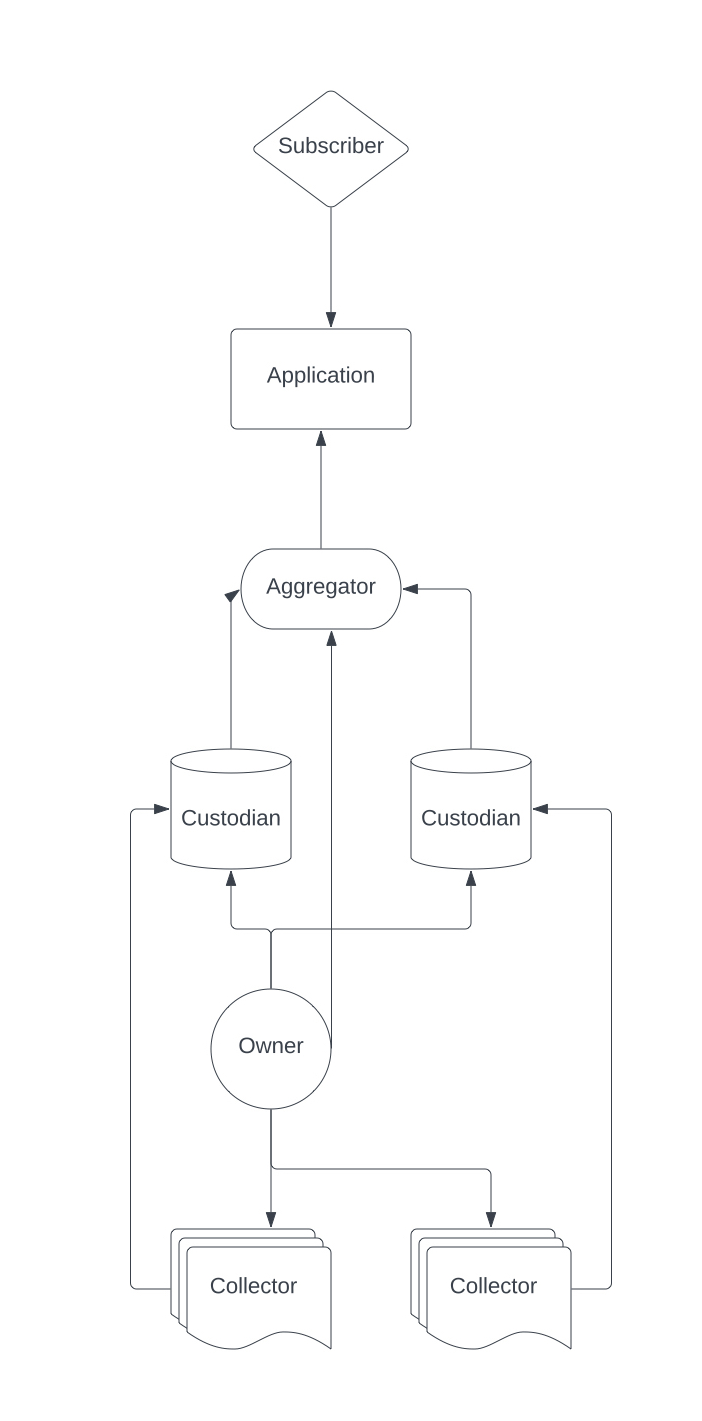
\includegraphics[width=170]{images/persona_strucutre.jpg}
    \caption{The flow of data in the data economy. The data is generated by the owner and flows from collectors to custodians to aggregators to applications and finally to the subscriber. The subscriber pays money that trickles back through the system. In order for the owner to actually have ownership of their data they must be able to manage the collector, custodian, and aggregator of their data.}
    \label{fig:DataActors}
\end{figure*}



\subsubsection{Actors in the Snickerdoodle Protocol}
% For our version 1 how are we going to break down the actors/personas
%     Individual's / end users
%.    Businesses
%     DAO
%.    SDL
We will simplify the actors for the initial version of the Snickerdoodle Protocol. The users of the protocol are data owners who will collect, store, and manage their data from a $\mathit{data wallet}$ (for more on data wallet, see \ref{section:DataWallet}). The data wallet will allow people to consent to aggregation and allow certain applications to run on their data by minting a non-transferable consent NFT (to learn more about the on-chain aggregation\&consent architecture and the applications, see sections \ref{section:Contracts} and \ref{section:SDQL} respectively). Lastly, consenting data wallets will send the resulting insights to an ingestion provider, which will allow businesses to see the insights they have paid for (see \ref{section:InsightService}). 


For implementation details check out section \ref{section:Implementation} and for ways we'll expand the protocol in the future check out section \ref{section:Future}.

\section{Implementation}
\label{section:Implementation}
%------------------------------------------------------------------------------------------
\subsection{Architecture}
\label{section:Architecture}

This section will discuss the implementation and design decisions of the Protocol. The Protocol has three primary 
components: a data wallet implementation, an on-chain data control plane, and aggregation service providers.

The data wallet is a software client that implements functionality which enables end-users to collect, index, and store their data as well as participate 
in the decentralized data network, see section \ref{section:DataWallet}. Organizations (consumers of data insights) will be able 
to query populations of data wallets through an on-chain control plane that adheres to a publish-subscribe (pub-sub) pattern, see section \ref{section:OnChain}. 

At the core of the control plane is an upgradable contract factory which produces independent instances of an EIP-721 compatible consent registry. 
Consent tokens claimed from these consent contracts are non-transferable but can be burned by the recipient. Claiming a consent token denotes a data 
wallet user's consent to participate in network queries in return for rewards (which may or may not be web3 digital assets). 

Data wallets receive queries via EVM events emitted from consent registry contracts they have claimed tokens in. These events contain metadata encoding
instructions (written in SDQL) to run computations on the data stored in the data wallet to produce insights. Once a data wallet has produced
the requested insight, it performs a digital "handshake" with the aggregation service provider specified in the query metadata such that the 
data wallet owner receives a reward while the requesting organization receives the insight, see figure \ref{fig:OnChainOffChain}. 

User consent and data flow is thus orchestrated in a distributed manner by the Protocol. It is also worth highlighting that while 
Snickerdoodle Labs will develop service infrastructure for the protocol (such as producing a data wallet and a SaaS product offering 
for enterprise participation in the protocol), the protocol itself is, however, permissionless and open so that anyone could implement a 
data wallet client or act as an aggregation service provider if the specifications of the protocol is adhered to. 
%----------------------------------------------------------------------------------------------------------------------------------------
\subsection{On-Chain Components}
\label{section:OnChain}

\subsubsection{Consent Contract Factory}
\label{section:ConsentFactory}

\begin{figure}[ht] 
    \centering
    % Define block styles
    \tikzstyle{decision} = [diamond, draw, fill=blue!20, 
    text width=4.5em, text badly centered, node distance=3cm, inner sep=0pt]
    \tikzstyle{daoblock} = [diamond, draw, fill=red!20, 
    text width=6em, text centered, rounded corners, minimum height=4em] 
    \tikzstyle{factoryblock} = [rectangle, draw, fill=blue!20, 
    text width=6em, text centered, rounded corners, minimum height=4em]
    \tikzstyle{instance} = [circle, draw, fill=violet!20, 
        text width=6em, text centered, rounded corners, minimum height=4em]
    \tikzstyle{line} = [draw, -latex']
    \tikzstyle{cloud} = [draw, ellipse,fill=red!20, node distance=3cm,
        minimum height=2em]
    
    \begin{tikzpicture}[node distance = 2cm, auto]
        % Place nodes
        \node [daoblock] (DAO) {Protocol DAO};
        \node [factoryblock, right of=DAO,  node distance=5cm] (FACTORY) {Consent Contract Factory};
        \node [instance, right of=FACTORY,  node distance=4cm] (CONTRACT2) {Consent Contract 2};
        \node [instance, above of=CONTRACT2,  node distance=3cm] (CONTRACT1) {Consent Contract 1};
        \node [instance, below of=CONTRACT2,  node distance=3cm] (CONTRACT3) {Consent Contract ...};
        % Draw edges
        \path [line] (DAO) -- node {upgrade} (FACTORY);
        \path [line] (FACTORY) |- node [near start, right] {deploy} (CONTRACT1);
        \path [line] (FACTORY) -- node [above] {deploy} (CONTRACT2);
        \path [line] (FACTORY) |- node [near start, right] {deploy} (CONTRACT3);
    \end{tikzpicture}
    \caption{The core of the on-chain protocol effectively implements an upgradeable, decentralized pub-sub 
    network. Insight consumers publish consent contracts via the consent contract factory and end-users subscribe 
    to consent contracts by claiming a non-transferable consent token.}
    \label{fig:ConsentFactory}
  \end{figure}
The on-chain components of the Protocol functions as a decentralized, permissionless data control plane. It specifically implements a publish-subscribe pattern
in which organizations publish new instances of an EIP-721 compatible consent registry (see \ref{section:ConsentContract}), and end-users 
subscribe to the registries by claiming a non-transferrable consent token. The publishing action is performed via the Protocol's upgradable 
consent contract factory, see figure \ref{fig:ConsentFactory}. The factory contract will be the entrypoint to the Protocol for new insight 
consumers, since a consent registry is required to communicate with the network of data wallets. 

\begin{figure}[ht] 
    \centering
    % Define block styles
    \tikzstyle{beacon} = [diamond, draw, fill=blue!20, 
    text width=6em, text centered, rounded corners, minimum height=4em] 
    \tikzstyle{proxy} = [rectangle, draw, fill=violet!20, 
    text width=6em, text centered, rounded corners, minimum height=4em]
    \tikzstyle{implementation} = [circle, draw, fill=violet!20, 
        text width=7em, text centered, rounded corners, minimum height=5em]
    \tikzstyle{line} = [draw, -latex', text width=5em]
    \tikzstyle{line2} = [draw, -latex']
    
    \begin{tikzpicture}[node distance = 2cm, auto]
        % Place nodes
        \node [beacon] (BEACON) {Upgradable Beacon};
        \node [proxy, right of=BEACON,  node distance=7cm] (PROXY) {Proxy Contract};
        \node [implementation, above of=BEACON,  node distance=7cm] (IMP1) {Old Implementation};
        \node [implementation, right of=IMP1,  node distance=7cm] (IMP2) {New Implementation};
        % Draw edges
        \path [line] (PROXY) -- node {implementation address?} (BEACON);
        \path [line] (PROXY) -- node [near start, right] {old call delegation} (IMP1);
        \path [line] (PROXY) -- node [right] {new call delegation} (IMP2);
        \path [line2] (BEACON) -- node [near start, left] {old reference} (IMP1);
        \path [line2] (BEACON) -- node [near start, right] {new reference} (IMP2);
    \end{tikzpicture}
    \caption{The upgradable beacon pattern was popularized by the Dharma protocol. It allows for many proxy contracts to be upgraded with a single
    transaction as well as for gas-efficient deployments of new proxy contracts. When a function call is directed at a proxy, the proxy retrieves the
    implementation address from the upgradeable beacon then delegates the function call to the contract at that address.}
    \label{fig:UpgradePattern}
\end{figure}
The consent contract factory exists as a utility for insight consumers to create new consent registries. The factory is implemented with an 
upgradable beacon pattern, see figure \ref{fig:UpgradePattern} to enable gas-efficient deployments and to allow for seamless extensions of functionality
via DAO proposals. 

\paragraph{Factory Pattern}
The factory pattern defines a smart contract which is responsible for creating other contracts. The Protocol uses the factory 
pattern to simplify the deployment of new consent registries and to give new insight consumers a single point of entry into the data network. 

\paragraph{Upgradable Beacon Pattern}
\label{section:BeaconPattern}

Consent registries are deployed as proxy contract instances that reference an upgradable beacon contract to obtain the correct address to delegate
function calls, see \ref{fig:UpgradePattern}. This upgrade pattern compliments the factory pattern by allowing for very gas-efficient deployments 
of new proxy instances. Proxy contracts only store storage variables and a pointer to their designated upgradable beacon contract. The upgradable 
beacon contract points to an implementation contract. The implementation contract contains all functions implementations as well as the storage
variable declarations that proxy contracts copy. 

A Protocol upgrade to the consent registry functionality requires that a new implementation contract first be deployed to the blockchain. Then a 
DAO proposal must be initiated to point the upgradeable beacon to the new implementation address. All previously deployed and newly created proxy 
consent contracts inherit the functionality (and any new storage variables) defined in the new contract.

The upgradeability pattern is based on EIP-1967 (CITE) and is implemented through OpenZeppelin libraries (CITE).

\subsubsection{Consent Registries}
\label{section:ConsentContract}

\begin{figure*}[H] 
    \centering
    % Define block styles
    \tikzstyle{decision} = [diamond, draw, fill=blue!20, 
        text width=4.5em, text badly centered, node distance=3cm, inner sep=0pt]
    \tikzstyle{factoryblock} = [rectangle, draw, fill=blue!20, 
        text width=6em, text centered, rounded corners, minimum height=4em]
    \tikzstyle{actorblock} = [rectangle, draw, fill=green!20, 
        text width=6em, text centered, rounded corners, minimum height=4em]
    \tikzstyle{contract} = [circle, draw, fill=violet!20, 
        text width=6em, text centered, rounded corners, minimum height=4em]
    \tikzstyle{aggregator} = [cylinder, 
        draw = violet, 
        text = black,
        cylinder uses custom fill, 
        cylinder body fill = magenta!10, 
        cylinder end fill = magenta!40,
        aspect = 0.2, 
        shape border rotate = 90]
    \tikzstyle{line} = [draw, -latex']
    \tikzstyle{onchain} = [draw=blue!50, thick, fill=blue!10, rounded corners, rectangle, text width=7em, text centered]
    \tikzstyle{offchain} = [draw=red!50, thick, fill=red!10, rounded corners, rectangle, text width=7em, text centered]
    
    \begin{tikzpicture}[node distance = 2cm, auto]
        % Place nodes
        \node [factoryblock,  node distance=5cm] (FACTORY) {Consent Contract Factory};
        \node [contract, below of=FACTORY,  node distance=4cm] (CONTRACT) {Consent Registry};
        \node [aggregator, below of=CONTRACT,  node distance=3.5cm] (AS) {Aggregator Service};
        \node [actorblock, right of=AS,  node distance=6cm] (DW) {Data Wallet};
        \node [actorblock, left of=AS,  node distance=6.5cm] (IC) {Insight Consumer};
        % Draw edges
        \path [line] (IC) |- node [near end, below] {publish contract} (FACTORY);
        \path [line] (IC) |- node [near end] {request for data event} (CONTRACT);
        \path [line] (DW) |- node [near end, above] {opt in} (CONTRACT);
        \path [line] (FACTORY) -- node {deploy} (CONTRACT);
        \path [line] (DW) -- node [above] {insight delivery} (AS);
        \path [line] (IC) -- node {insight visualization} (AS);
        % On-Chain Box
        \begin{pgfonlayer}{background}
          \node[onchain, label={On-Chain}] [fit = (FACTORY) (CONTRACT)] {};
        \end{pgfonlayer}
        % Off-chain Box
        \begin{pgfonlayer}{background}
          \node[offchain, label={Off-Chain}] [fit = (IC) (AS) (DW)] {};
        \end{pgfonlayer}
    \end{tikzpicture}
    \caption{Insight consumers reach data wallet users by broadcasting events from a consent registry instance. Only data wallets that have
    claimed a non-transferrable consent token listen for events and deliver insights to the aggregation service URL listed in the associated
    request-for-data event.}
    \label{fig:OnChainOffChain}
  \end{figure*}
Consent registry contracts are the primary on-chain mechanism by which insight consumers interact with with data wallet end-users. Consent 
registries allow organizations to create data pools by serving as an on-chain data structure that holds metadata regarding the conditions 
under which data is to be collected and used as well as a cryptographically verifiable list of externally owned accounts (EOAs) that have
have given consent to participate in the data pool. 

Consent registries expose an EIP-721 compatible interface. This is for developer integration convenience as it allows consent registries to 
be readable by most existing NFT indexing services (such as Snowtrace). Consent is denoted by ownership of a non-transferrable consent NFT 
(non-fungible token) which can be burned by the owner at any time. 

\paragraph{Request for Data Events}


After an organization has published a consent registry via the Consent Contract Factory (see \ref{section:ConsentFactory}), the organization can emit
EVM events by calling a special function, $requestForData$, which takes a content identifier (CID) as its only input. This CID is used to 
retrieve the request specifications from a suitable content addressable network (like IPFS) that the data wallets will process. Data wallets can detect 
past $requestForData$ events by constructing EVM query filters and requesting all EVM logs that match those filters. Thus consent registries offer a 
tamper-resistant communication layer between organizations and participants in their data pools. See figure \ref{fig:OnChainOffChain}

Consent registries also specify a $queryHorizon$ which inform data wallets of the oldest block number to search for these events. This variable is 
first initialized to the block number that the proxy contract was deployed from the contract factory and can be updated by an EOA with the $DEFAULT\_ADMIN\ROLE$
to a later blocknumber (but cannot be changed to an earlier block number). Setting a reasonable value for $queryHorizon$ is important since many RPC providers
only allow for query filters to search a limited history of the chain.

\paragraph{User Data Permissioning}

A $requestForData$ event indicate that it requires access to multiple attributes indexed by the user's data wallet client, such as country of origin, age,
on-chain contracts they have interacted with using their linked EOA asset account. However, users can set granular permissions regarding their indexed data 
attributes. 

Every consent token issued from a consent registry has an associated set of binary $aggreementFlags$. There are 256 flags in total (the size of an EVM word) 
though not all flags will be assigned to specific attributes at Protocol launch, leaving room for customization. Only the owner of a consent token can 
update the granular permissions denoted by the token's $agreementFlag$s. The availability of granular consent data on-chain allows organizations to better 
understand what kinds of insights they will be able to obtain from their data pool before calling $requestForData$. 

\paragraph{Consent Invitations}
\label{section:ConsentInvitations}


Consent registry metadata is used for the decentralized, trustless, and tamper-resistant triggering of user flows that should be presented to the data wallet 
end user in a format appropriate for the data wallet client environment. In a web browser setting, the data wallet detects the current active URL, and via DNS 
over HTTPS (DoS) queries the TXT records associated with the apex domain. If the TXT record contains a reference to a Protocol consent 
contract address, the data wallet then fetches the URLs registered in the consent registry $domains$ metadata storage variable and cross-references the domains 
listed from the contract to the current URL. If the data wallet detects that the current URL is included in the domains listed in the 
consent contract, the data wallet will inject a user flow into the browser DOM. The content of the user-flow is fetched from the URL specified by the consent 
registry $baseURI$ parameter. 
\begin{figure*}[!htbp] 
    \centering
    \tikzset{
    state/.style={
           rectangle,
           rounded corners,
           draw=black, very thick,
           minimum height=2em,
           inner sep=2pt,
           text centered,
           },
}

\begin{tikzpicture}[->,>=stealth']

 % Position of QUERY 
 % Use previously defined 'state' as layout (see above)
 % use tabular for content to get columns/rows
 % parbox to limit width of the listing
 \node[state,
 anchor=center] (DATA WALLET) 
 {\begin{tabular}{l}
  \textbf{Data Wallet}\\
  \parbox{7cm}{
  Web3 Invitation Popup Protocol
  \begin{enumerate}
   \item Detect Environment State Change
   \item Scan for contract address tag
   \item Read URIs from contract
   \item Assert tag/URI aggreement
   \item Trigger Invitation on successful assert
  \end{enumerate}
  }\\[5em]
 \end{tabular}};
  
 % State: ENV with different content
 \node[state,    	% layout (defined above)
  text width=7cm, 	% max text width
  above of=DATA WALLET, 	% Position is to the right of QUERY
  node distance=6.5cm, 	% distance to QUERY
  ] (ENV) 	% posistion relative to the center of the 'box'
 {%
 \begin{tabular}{l} 	% content
  \textbf{Environment State (Off-Chain)}\\
  \parbox{7cm}{
  Contract tag examples:
   \begin{enumerate}
     \item TXT Record (web/mobile browser env)
     \item Meta tag (web/mobile browser env)
     \item hidden file (native app env)
     \item application event (native/browser env)
  \end{enumerate}
  }
 \end{tabular}
 };
 
 % STATE CONTRACT
 \node[state,
  right of=DATA WALLET,
  node distance=9.5cm,
  text width=6cm] (CONTRACT) 
 {%
 \begin{tabular}{l}
  \textbf{Consent Contract (On-Chain)}\\
  \parbox{6cm}{
  On-Chain URI examples:
      \begin{enumerate}
        \item Web URL
        \item application signature
      \end{enumerate}
  }
 \end{tabular}
 };


 % draw the paths and and print some Text below/above the graph
 \path (DATA WALLET) 	edge[bend left=20]  node[anchor=west,left]{$1$} (ENV)
 (ENV) 	edge[bend left=20]  node[anchor=east,right]{$2$} (DATA WALLET)
 (DATA WALLET)     	edge[bend left=20] node[anchor=north,above]{$3$} (CONTRACT)
 (CONTRACT)     	edge[bend left=20] node[anchor=south,below]{$4$} (DATA WALLET)
 (DATA WALLET) 	edge[bend right=30]  node[anchor=east,right]{$5$} (ENV);

\end{tikzpicture}
    \caption{Actor model of the tamper-resistant web3 invitation popup protocol.}
    \label{fig:PopupProtocol}
  \end{figure*}
The Web3 popup protocol can be extended to other environments including mobile browsing environments, VR experiences, gaming consoles, etc as indicated by 
figure \ref{fig:PopupProtocol}. The user flows presented by these tamper-resistant popups serve as the on-boarding mechanism for end-user's to opt into a data pool.

\paragraph{Opt-In methods and Meta-Transactions}

The consent registries have to modes by which user's can join a data pool: open-access and invite-only. Consent registries in which open-access is 
enabled ($openOptInDisabled$ is $false$), any EOA is allowed to claim a consent token by calling the $optIn$ method and paying the associated gas
fees. Registries where $openOptInDisabled$ is $true$ are invite only and require a signature for an EOA with the $SIGNER\_ROLE$ in order to join 
a data pool. There are two available methods for invitation-only user opt-in: $restrictedOptIn$ and $anonymousRestrictedOptIn$. The former method
requires that the recipient EOA be known in advance by the $SIGNER\_ROLE$ in order to construct the appropriate signature. The receiving EOA then 
becomes the only account that can call $restrictedOptIn$ with that signature. If the recipient EOA address is not known ahead of time, the $SIGNER\_ROLE$
can construct a signature for use with the $anonymousRestrictedOptIn$ method in which any EOA can submit the signature to that method (a single time) 
in order to opt-in. 

Support for both open and invitation-only opt-in flows makes the Protocol flexible to a variety of use-cases. However, end users are often hesitant to 
spent their own cryptocurrency in order to pay for transaction fees associated with a decentralized application or simply do not have the tokens 
necessary to do so. Additionally, requiring the user to spend their own assets to participate in the Protocol intoduces significant user friction and
adoption hurdles. Consent registries implement EIP-2772 compatible metatransaction capabilities to circumvent this issue. 

Meta transactions allow someone else to pay for a user's gas fees. All opt-in methods will implement support for metatransactions. This will offer the 
flexibility to have users pay for their own gas or have the businesses pay.  

\subsubsection{Identity Crumbs}
\label{section:Crumbs}

The Protocol introduces a special EIP-721 compatible registry, called the Crumbs Contract, to facilitate data wallet synchronization when an end user 
installs the client on a new device. When a user links a new EOA to their data wallet identity, the EOA encrypts their data wallet identity EOA (see section
\ref{section:DataWalletIdentity}) and stores the encrypted data in the token URI of an entry in the Crumbs contract. 

During a new client installation, the end user must simply link any EOA that has previously been linked to their data wallet identity in order for the data 
wallet to synchronize from their previously saved state that has been stored in the decentralized persistence layer of the data wallet network. The data wallet
checks if the account being linked owns a token in the Crumbs contract; if so, it reads the encrypted content of the token URI, decrypts the information, and loads 
the public-private key pair into memory. 

\subsubsection{EIP-20 Token}
\label{section:Token}
The Protocol includes a fungible utility token adhering to the EIP-20 standard. This token will be used for paying various fees required to leverage
the Protocol (like publishing a new consent registry) and will also be used for voting in the Protocol DAO. The associated voting mechanism that 
accompanies the possession of a token can be delegated to a different address without relinquishing ownership of the token

\subsubsection{Decentralized Autonomous Organization}
\label{section:ImplementationDAO}

The Protocol will include a decentralized autonomous organization (DAO) implementation. The DAO will be responsible for proposing and executing upgrades to 
the Protocol. The particular pattern used by the Protocol DAO is based on Curve Finance's DAO and will be implemented with OpenZeppelin libraries. 

Token holders (see section \ref{section:Token}), are responsible for the creation and execution of DAO proposals. At mainnet launch it is anticipated that one 
token will render one vote, though this too could be modified via a DAO proposal. Token holders will have to reach a pre-specified quorum of voting power in 
order to successfully create a proposal in the DAO task queue. Successful proposals will be subject to a delay of at least one block before they can be executed 
in order to prevent flash loan attacks. 

%----------------------------------------------------------------------------------------------------------------------------------------
\subsection{Data wallet}
\label{section:DataWallet}

\begin{figure*}[!htbp] 
    \centering
    \begin{tikzpicture}[
      scale=0.75,
      start chain=1 going below, 
      start chain=2 going right,
      node distance=1mm,
      desc/.style={
        scale=0.75,
        on chain=2,
        rectangle,
        rounded corners,
        draw=black, 
        very thick,
        text centered,
        text width=8cm,
        minimum height=12mm,
        fill=purple!60
        },
      it/.style={
        fill=violet!20
      },
      level/.style={
        scale=0.75,
        on chain=1,
        minimum height=12mm,
        text width=2cm,
        text centered
      },
      every node/.style={font=\sffamily}
    ]
    
    % Levels
    \node [level] (Level 5) {Presentation Layer};
    \node [level] (Level 4) {Identity Layer};
    \node [level] (Level 3) {Events Layer};
    \node [level] (Level 2) {Execution Layer};
    \node [level] (Level 1) {Permissions Layer};
    \node [level] (Level 0) {Data Layer};
    
    % Descriptions
    \chainin (Level 5); % Start right of Level 5
    % application layers
    \node [desc, it] (Form) {Application and Form Factor Logic};
    \node [desc, it, continue chain=going below] (Identity) {Signature Verification and Identity Creation};
    % protocol layers
    \node [desc] (Events) {Environment and Protocol Event Detection};
    \node [desc] (Execution) {Query Interpretation and Execution};
    \node [desc] (Permissions) {Granular Attributed-Based Access Control};
    \node [desc] (Data) {Indexing/Storage/Synchronization of Web2/Web3 Data};
    
    \end{tikzpicture}
    \caption{Logical structure of a protocol data wallet.}
    \label{fig:DataWalletStructure}
  \end{figure*}

\input{InsightControlFLowTikz}

The data wallet is the primary end-user client interface within the Protocol. It enables data ownership by facilitating user control 
and consent to the collection, storage, and usage of their data. The data wallet should provide the following functionality:
\begin{itemize}
  \item Secure storage of the data
  \item A query engine for individualized data mining
  \item Aggregation and indexing of user data. This should include on-chain data, data from traditional third-party sources, or digital identities.
  \item A consent management interface for granular access control
  \item Localized insight processing and submission
  \item Reward discovery and management
  \item Identity and verifiable credential management
\end{itemize}

To the user, the data wallet operates in a conceptually similar way to a conventional cryptocurrency wallet, but with a wider scope. 
Instead of key and account management of a blockchain account, a data wallet manages the storage, collection, and sharing of insights derived 
from user data. The initial form factor will be a stand-alone browser extension with plans to expand the form factor in future versions (see 
section \ref{section:FormFactor}). By providing this localized control interface, the data wallet will give individuals greater control 
of their own data and allow for participation in the Protocol.

\subsubsection{Storage}

Secure storage of data is crucial to allowing people to own their data. The initial data wallet implementation produced by 
Snickerdoodle Labs will expose a modular storage interface capable of integrating with various storage provider technologies, 
such as Google Storage, Amazon S3, or decentralized options like the Ceramic Network.

It is also important to call out the wallet's storage of public-private key pairs. A data wallet should only store public keys 
and digital signatures associated with accounts linked to a user's data wallet, not private keys. 
Instead, we integrate with existing wallets (e.g., MetaMask) for key management.


\subsubsection{Collection}
The data wallet will also help users own their own data by allowing them to collect the data that they generate. This individualized data mining 
provides highly accurate data that the protocol allows users to easily monetize. The data the wallet collects has three important properties: 
explicit/implicit, first/third party, and authenticated/unauthenticated. %Not sure if there's a better term

% should be included but I'm not sure where or how
An important feature to highlight is that multiple addresses can be linked together in the same data wallet, including wallets for separate chains. 

% Not sure if this should be a paragraph or points
\paragraph{Explicit/Implicit}
The data wallet will either collect data through explicit or implicit means. Explicit data is data directly provided by the user, such as their name, 
age, or wallet address. In the initial version of the data wallet, the user will manually input this data; however, in the future, the data wallet 
could feature in-browser event capturing to passively collect this data (e.g., collecting information about what websites a user has visited).


Implicit data is data generated by user action. For example, using a user's wallet address to learn that they swapped specific tokens or have played a web3 game. 


\paragraph{First/Third Party}
Data collected can come from different sources. Specifically, first-party data comes directly from the user, and third-party data comes from 
someone other than the user. For example, if the user directly inputs their name, their name would be considered first-party data; if the 
user imports their name from the DMV, that would be third-party data.


\paragraph{Authenticated/Unauthenticated}
Data can be authenticated if its origin and validity can be verified through cryptographic means and unauthenticated if it can't. For example, 
a wallet address can be authenticated if we receive a signed message from that address. Third-party data can be authenticated if it has a known 
identity (e.g., the DMV's public key is known, and the data wallet receives data signed by that key). 

\subsubsection{Localized Processing} % listens to events and processes queries

The data wallet is a local application that stores the owner's data securely and processes computations locally. By collecting and 
securely storing user data locally, the data wallet guarantees data ownership to the user by never sharing it. Because computations 
are running locally, the owner ensures that only analysis they've given consent to can run on their data. Businesses also benefit 
from this model as they can leverage data-driven insights without worrying about the liability or infrastructure of storing raw, 
personal data. While the initial version of localized processing will be more limited, there is a myriad of ways we can modify this 
approach to add additional data safety and features (see section \ref{section:Future}). 

The wallet will learn what computations to run by listening to on-chain events. These events will be emitted on the Snickerdoodle Avalanche 
subnet and specify SDQL queries that include the computation instructions. If those data request events are from consent contracts that the 
user has opted into, the data wallet will process the data following the rules in the associated SDQL query. After the localized processing 
has been completed, the data wallet will send the insights to the specified endpoint, and the data owner will collect any rewards.


\subsubsection{Snickerdoodle Query Language} % maybe move to contracts 
\label{section:SDQL}

The Snickerdoodle Query Language will allow businesses to share their data requests with individual users in a transparent and auditable fashion. 
It will be structured as a simple JSON file containing information on the eligibility requirements, rewards, data to be collected, what processing 
to perform, and where to send processed data (see figure TODO). The allowed functions and syntax of the language will be enforced by the 
Snickerdoodle DAO and determined by token holders, which will allow for its continued development and the enforcement of user privacy. SDQL 
queries must be stored on a content-addressable distributed network, such as IPFS, to ensure tamper resistance. 

TODO FIGURE SHOWING QUERY + flesh out sections


\subsubsection{Rewards}

An essential part of the protocol is allowing individuals to get value from their rewards. The data wallet will facilitate this by allowing users 
to gain rewards for sharing their data. First, the data wallet helps people find rewards that are being offered. If a person goes to a website 
that's enabled the Snickerdoodle Protocol, they will see a pop-up and can connect their data wallet to check out possible rewards. Additionally, 
the data wallet will have a section showing available rewards.


Once the user has given consent to share data, the data wallet will also help the user manage their rewards. When they receive a query, they will 
be able to visualize the rewards offered in that query. The owner will also be able to set which addresses and chains they want to receive rewards. 
Additionally, the owner will be able to see the history of the rewards they've received and the data exchanged. 

\subsubsection{Authorization and Consent Management}

Enabling informed consent for data sharing is a core function of the Snickerdoodle Protocol. Consent is accomplished through the use of consent contracts 
(see section \ref{section:Contracts}). When a user wishes to consent to share data, they make a contract call and are issued a non-transferable consent 
token. To revoke consent, they can burn that token. The data wallet facilitates this by giving the owner's crypto wallet the appropriate transactions to 
sign. Once opted in, the data wallet will respond to all eligible queries from that pool unless more granular data permissions have been specified within 
the wallet. TODO granular permissions
%TODO granular permissions and opting out


For the initial version of the Snickerdoodle Protocol, we are not allowing users to choose what types of queries they can opt in and out of. A user giving 
consent to a company allows that company to run any query on their data. However, to maintain privacy, we limit queries' interactions with PII. If any 
queries touch-sensitive data, we will reduce the resolution of the insight, e.g., location data will only reveal the state or country, not the zip code. 
Additionally, part of the design of the data wallet is that it has the final say on what data is shared. Even if a user consents to a consent contract, a 
data wallet can theoretically choose not to respond, making it easy for future versions of the wallet to enable more granular privacy controls.

\subsubsection{Distributed Runtime Library}

The distributed runtime library is a core security feature of the data wallet. The wallet browser plugin will leverage iFrames to run plugins for data 
processing and wallet integrations. Using iFrames like this will isolate the data wallet's processing from the browser. To ensure the validity of these 
plugins, we will use the iFrame to enforce the legitimacy of the code by verifying certificates and checksums with the DAO allowlist. In this way, the 
user has a trustless way to verify their data is being processed and held safely.

\subsubsection{Queries}

Queries are responsible for specifying the who, what, and why of data processing. They allow data subscribers to define who they want data from, what type 
of computation to run, where to send the insight, and the reward for sending the insight. These queries must be content-addressed, so anyone can access the 
query and verify its validity. For the initial version of the Snickerdoodle Protocol, we will be publishing these queries on IPFS. In the future, the protocol 
will support queries hosted through other means.

TODO add info only allow queries if there are 30+ consent tokens given out

\subsubsection{Network \& Fees}

The Snickerdoodle Protocol will be deployed on the Snickerdoodle Network, which will be an EVM-compatible Avalanche Subnet. Our requirements for the 
network were we wanted a scalable network with low fees and EVM compatibility. Making an Avalanche Subnet fit these requirements (IDK more and IDK the how).

As mentioned in \ref{section:DoodleToken}, the native token of this subnet will be the Doodle and will be used for paying fees. Within the context 
of the protocol and managing data, gas fees will be paid for creating consent contracts, creating consent tokens, and emitting events (i.e., SDQL queries). 
Data subscribers will pay additional protocol fees to emit an SDQL query to access insights. This protocol fee will be proportional to the amount of data 
being accessed and can be calculated using the number of consent tokens tied to a specific contract.

\subsubsection{Rewards}

After sharing insights, the protocol will facilitate the transfer of rewards to the data owner. The owner can choose which wallet to send rewards to, not 
just the data wallet. In the initial version of the protocol, the insights/rewards transfer process will be trust-centric. When an owner responds to a 
query, they must trust that the business will send them the reward later. When subscribers send a reward, they need to trust that the user is sending 
over authentic insights. In future versions, we will enable atomic reward swaps. Atomic swaps allow insights to be shared at the same instance that a 
reward is received. We could easily add this functionality if the rewards are in DOODLE tokens, and zero-knowledge proofs could enable atomic swaps 
with different assets across chains (see \ref{section:AtomicSwaps}).

\subsubsection{Privacy}

A user receiving a consent token is how users signal their consent and a business emitting an event is how they signal they are interested in a particular 
insight. This transparency in knowledge does come with some privacy tradeoffs:
\begin{itemize}
  \item Everyone knows who is giving consent to a business
  \item Everyone knows what queries a business has run
\end{itemize}

These privacy trade-offs are acceptable for the initial version of the protocol. Our goals are to make sure users are able to give informed consent to the 
use of their data, data isn't revealed if this consent isn't given, insights rather than raw data are revealed if consent is given, and businesses will pay 
more to send queries to more people. The use of public consent tokens allows us to achieve these goals with an acceptable amount of privacy. It also gives 
the initial version of the protocol an interoperability bonus by allowing the consent tokens to integrate with existing web3 solutions. By making consent a 
public token that conforms to the ERC-721 standard, people can see what they've consented to through any application that shows owned NFTs. In a future 
version, we could create ways to hide this information. For example, an anonymized consent token could be minted while the data wallet listens and responds 
to events. %TODO maybe reference future


It's also worth pointing out that this decision doesn't reduce the privacy of individuals too much more than if we didn't use public consent tokens. Accepting 
rewards linked to a business reveals that consent has been given to that business (i.e., Alice having a Bob's Business NFT means everyone knows Alice consented 
to provide information to Bob's Business). Additionally, there will be a limited number of subscribers for the initial release, all of which will be web3 
companies. This limitation reduces the information revealed by owning a token. Holding a consent token for a particular business indicates interaction with 
the business and the willingness to adopt a web3 product for a reward. The former is already public knowledge by looking at the blockchain's history, and the 
latter is a common trait of web3 users.


We are also ok reducing businesses' privacy by making what queries are run public. We feel that more transparency in what information businesses are interested 
in gives people more insight into whether they want to share their data and reduces the societal risk of companies running complex insights that hurt the 
commonwealth. If we need to add more privacy to businesses, we could add it in future versions by creating private query cohorts. See section \ref{section:Future} 
for a discussion on future changes to the protocol that can increase privacy.

\subsection{Data Ingestion Provider} % name for role?

Data ingestion is the final stage of the insight aggregation process that allows subscribers to access the insights generated at the data wallet layer. 
This section will detail how the subscriber can see processed data from the user's data wallet. Any entity can assume the role of data ingestion service 
as long as they follow the protocol and are accepted by the DAO. Snickerdoodle Labs will offer the first data ingestion provider, which will be tied to 
a SaaS product. 

\subsubsection{Ingestion}
The final step of the protocol is for data wallets to send insights from their queries to an endpoint. This endpoint is the ingestion provider and is 
specified in the SDQL query. Ingestion is an integral part of the protocol as it allows businesses to see the insights they have paid for.

Once the ingestion provider receives the insight, it must store the insights events and manage access. They can also provide any additional services 
they want on top of this, such as providing a dashboard to view insights. There is no way to mathematically guarantee any ingestion provider is behaving 
honestly or doesn't have any bugs. The lack of a strong guarantee means that actors in the protocol have to put some trust in ingestion providers. The 
Snickerdoodle Protocol reduces this problem by only allowing ingestion services that the DAO has approved. Any provider has to be trustworthy enough for 
the DAO to vote them in; if a provider is revealed to be a bad or incompetent actor, they can be voted out. For a deeper discussion of data safety 
concerns with ingestion providers, see section \ref{section:IngestionDataSafety}.

\subsubsection{Data Safety}
\label{section:IngestionDataSafety}

The initial version of the protocol requires trust in the Insight Platform to maintain data safety. As discussed above, there are no guarantees that the 
ingestion provider acts honestly. The ingestion provider can see, delete, and sell any insights they receive. Additionally, because the initial version 
of the wallet only implements simple anonymization techniques, ingestion providers could identify who shared the insight and reconstruct the raw data. 


To reduce these privacy risks, the initial version of the protocol will only allow queries that don't reveal PII, and future versions will add anonymization 
techniques to insight computations (see section \ref{section:Future}). To reduce the risk of malicious ingestion services, the Snickerdoodle DAO will maintain 
an allowlist of trusted actors. Additionally, Snickerdoodle Labs will be providing an ingestion service. The Snickerdoodle Ingisht Service is a SaaS product 
that will enforce data safety and has a massive financial and legal incentive to behave honestly.

\subsubsection{SDL Insight Platform}
\label{section:InsightService}

The Snickerdoodle Insight Platform will be our SaaS product offering for interaction with the Snickerdoodle Protocol. The Insight Platform will provide an 
ingestion service and help manage interaction with the rest of the protocol. This includes support for creating and managing queries, consent contracts, 
rewards, and website integrations. The Insight Platform will also provide an analytics dashboard to help businesses see their insights.
\section{Tokenomics}
\label{section:tokenomics}

\begin{figure}[!ht] 
    \centering
    \smartdiagram[circular diagram:clockwise]{DAO, Project Proposals, Exchanges, Protocol Users}
    \caption{Lifecycle of the Protocol token.}
    \label{fig:Tokenomics}
\end{figure}

The Protocol will issue a fungible token on mainnet launch, the technical aspects of which are given in section \ref{section:Token}. The token will serve both network governance and protocol utility purposes outlined in the following subsections. 

\subsection{Governance}
\label{section:Governance}
A fundamental use case the Protocol token will be network governance. At mainnet launch, it is anticipated that one token will be eligible to cast one vote in active DAO proposals. Token voting weight could be upgraded via future DAO proposals. For implementational details about the logical structure of the Protocol DAO, see section \ref{section:ImplementationDAO}.

Protocol contract upgrades will be executable only via DAO proposals. The upgrade pattern used by the Protocol is the upgradeable beacon pattern, see section \ref{section:BeaconPattern}. DAO proposals would be capable up updating the implementation address of Protocol beacon contracts in order to augment or introduction new on-chain functionality.

Lastly, it is anticipated that the DAO will function as a decentralized treasury, accumulating tokens spent during the utilization of the Protocol. DAO proposals can be 
created to allocate these funds in a manner appropriate for the furthering of the Protocol as depicted in figure \ref{fig:Tokenomics}.

\subsection{Utility Functions}
\label{section:TokenUtility}

It is anticipated that the Protocol token will have several utility use cases for initiating certain activities within the on-chain mechanics of the Protocol (see section \ref{section:OnChain} for details of on-chain components). It is desired by the Protocol designers that the token accrue value as the size of the data set represented by all data wallet users grows. The following mechanisms are likely to be implemented as on-chain logic in order to facilitate this goal:

\paragraph{Factory Fees}
The consent contract factory (section \ref{section:ConsentFactory}) will possibly require that token be spent in order to deploy a new consent registry. It is thought that requiring a token fee to publish a consent registry will disincentivize fragmentation of the data network, since it will be more expense to create multiple data pools than a single data pool. The token spent would be routed to the DAO treasury address. The fee amount would be set by DAO proposals. 

\paragraph{Request-for-Data Fees}
In order to disincentivize frivolous $requestForData$ events, it is anticipated that there will be a token fee
required to emit these events. The fees could be a fixed cost or proportional to the number of consent tokens
issued in the consent registry at the time of the function call. The token spent would be routed to the DAO treasury address. The fee amount and structure would be set by DAO proposals. 

\paragraph{Stake for Ranking}

In the scenario where there are many consent registries published by many different organizations for varying purposes, it will be necessary to have a built-in search mechanism to enable data wallet users to find data pools that fit their interests. The Protocol may introduce a staking registry where consent registry
publishers stake token in order to boost their indexed ranking in the list. This could be further granularized by introducing different verticals that stake could be allocated towards (some examples could be gaming, trading, consumer products, etc.). Data wallet implementations could leverage this staked ranking registry in order to present appropriate data pools to users based on the content of the data stored in their wallets. 

Organizations could reclaim their staked token when a boosted ranking is no longer relevant for their consent registry, with some fraction of the token held back for the DAO treasury. Staking organizations that abuse the ranking system would be at risk of having their stake forfeited to the DAO treasury in its entirety and the ranking eliminated by a DAO proposal. 

\subsection{Token Distribution}
\begin{figure}[!ht] 
    \centering
    \def\angle{0}
    \def\radius{3}
    \def\cyclelist{{"orange","blue","red","green","violet"}}
    \newcount\cyclecount \cyclecount=-1
    \newcount\ind \ind=-1
    \begin{tikzpicture}[nodes = {font=\sffamily}]
    \foreach \percent/\name in {
          30/Foundation,
          25/Token Sales,
          20/SDL Reserve,
          17/Team and Seed Investors,
          8/Future Employees of SDL
        } {
          \ifx\percent\empty\else               % If \percent is empty, do nothing
            \global\advance\cyclecount by 1     % Advance cyclecount
            \global\advance\ind by 1            % Advance list index
            \ifnum4<\cyclecount                 % If cyclecount is larger than list
              \global\cyclecount=0              %   reset cyclecount and
              \global\ind=0                     %   reset list index
            \fi
            \pgfmathparse{\cyclelist[\the\ind]} % Get color from cycle list
            \edef\color{\pgfmathresult}         %   and store as \color
            % Draw angle and set labels
            \draw[fill={\color!50},draw={\color}] (0,0) -- (\angle:\radius)
              arc (\angle:\angle+\percent*3.6:\radius) -- cycle;
            \node at (\angle+0.5*\percent*3.6:0.7*\radius) {\percent\,\%};
            \node[pin=\angle+0.5*\percent*3.6:\name]
              at (\angle+0.5*\percent*3.6:\radius) {};
            \pgfmathparse{\angle+\percent*3.6}  % Advance angle
            \xdef\angle{\pgfmathresult}         %   and store in \angle
        \fi
        };
    \end{tikzpicture}
    \caption{Protocol token distribution breakdown. The total supply is capped at 13.5 billion.}
    \label{fig:TokenDistribution}
\end{figure}
The Protocol token (section \ref{section:Token} is capped to a total of 13.5 billion. The allocation of the token supply is given in figure \ref{fig:TokenDistribution}. The Protocol Foundation will be allocated the largest percentage of the supply at the time of token generation with Snickerdoodle Labs (SDL) receiving 20 percent of the supply.
\section{Future Considerations}
\label{section:Future}
% make sure we highlight problems we referenced earlier in paper
The First version of the Snickerdoodle Protocol won't be able to achieve everything we aim to achieve. This section will detail potential improvements we can make to the protocol and potential risks the protocol faces.

\subsection{Potential Improvements}
This section will deal with potential improvements we can make to the protocol. Many of the changes are related but each change can be made independently.  

\subsubsection{Data Sharing}
% Federated Learning
% Perturbation Techniques (Differential Privacy)
%       Could solve privacy issue with ingestion
% Anonymization Techniques 
%       Could solve privacy issue with ingestion
% Multi-Party Compute
% Compute-to-Data
% private query cohorts / private groups
Currently, the protocol enables a basic version of data sharing, where only a simple set of predefined functions can be run on an individual's data and shared with one subscriber. An easy way to improve the protocol would be to enable more possible functions to run on this compute-to-data model. The currently allowed functions can only be run on a single individual's data. We could extend the protocol to run functions on multiple people's data before returning, thus enabling Multi-Party-Compute. Data is also only allowed to flow from data wallets to ingestion providers. Instead, we could create a back and forth between the data wallet and the subscriber. Allowing this back and forth would enable us to create a system to support federated learning. The subscriber would send over a pre-trained model, the wallet would update the model and send it back, and then the subscriber could combine the updates from every wallet and repeat the process.
Additionally, we can make changes to improve the privacy of the protocol. We could have the wallet use different anonymization techniques to prevent the wallet from sending PII to the insight service. Similarly, the wallet could expand its use of perturbation techniques and differential privacy. We can also add changes to how the protocol gets queries from the content addressing network to hide what queries subscribers are running. For example, we could create private query cohorts, so only a subset of the network knows what questions a business is interested in.

\subsubsection{Atomic Reward Swaps}
\label{section:AtomicSwaps}
The initial version of the protocol involves a trust-centric rewards-sharing mechanism. Ideally, there would not be any trust involved. The data owner only shares their insight once they know they will get a reward. The data subscriber will only send the rewards once they know they will receive a valid insight. One way to solve the transfer problem is with Zero-Knowledge atomic swaps (CITE). Only when both sides can guarantee that a valid trade will happen will insights and rewards be exchanged. We can also extend atomic swaps to cross-chain interactions. For a discussion on ensuring that insights are valid, see section \ref{section:DataOutsourcing}.

% https://ieeexplore.ieee.org/document/9181875
% https://eprint.iacr.org/2022/717.pdf
% https://patentscope.wipo.int/search/en/detail.jsf?docId=SG253980096&docAn=10201903150Q

\subsubsection{Cryptography}
% ZK-proofs
%   Could solve rewards issue
% Signing Scemas
% Data-Leasing
% Data Tracking
%   proof of storage
%   proof of deletion (lol)
The ability to update the cryptography is built into the Snickerdoodle Protocol because it is essential to patch security holes. This same idea allows us to add new cryptography that can enable new ways for the system to provide data safety guarantees. 

This wouldn't be a web3 white paper if we didn't mention how ZK-proofs could improve our system (lol this can be removed). ZK-proofs could allow data wallets to get consent tokens or rewards without others in the network knowing. Introducing new signing schemas will enable us to create proper data fiduciaries who can safely allow individuals to delegate their consent to others. Some interesting cryptography may enable data to be leased by only allowing decryption for a set amount of time. Additionally, we can use different cryptographic ideas to increase data tracking of data custodians (e.g., proof of storage and proof of deletion).

\subsubsection{Data Outsourcing}
\label{section:DataOutsourcing}
% Third-Party Implicit data (Collectors / EXtractors)
%   - Authorized Data Providers / Signers
% Data Custodians
% Data Fiduciaries
%   - Data unions
% Query Functionality
%   - Governance
%   - Permission Models (we might already have)
%   - Data Schemas
%   - Query Functions

% TODO this section is especially rough
Another avenue we want to look at for increasing the protocol's usefulness is increasing the amount of data that the protocol can collect. We can do this in several ways: enabling third-party verified data (e.g., DMV signed driver's license), expanding the data wallet to allow other methods of storage (e.g., delegating my personal Dropbox to store data on my behalf), and creating better ways for individuals to combine their data preemptively to create data unions. 

Lastly, we can improve a vast amount of functionality by increasing what can be managed on-chain by the DAO. We can add more query functions. We can also update the output of queries to update what data ingestors. And we can create a way to manage data schemas collected by verified third parties. 

\subsubsection{Form Factor}
\label{section:FormFactor}
%   - MOBILE
%   - Headless
%       - IOT
%   - Interobability 
%       - Chain agnostic
The Snickerdoodle Protocol can also update its form factor. We can make it so the protocol can work across chains. (maybe something about oracles with rewards and EVM compatibility). We can make the protocol work on headless browsers so it can live on IoT devices. We can also move the data wallet onto mobile, which is a natural extension given how much personal data individuals generate on mobile devices.

\subsection{Potential Risks}
This section will detail risks with the protocol we are worried about and hope to address. These risks include worries about market adoption, security of the protocol, privacy, and equity of data as an asset.

\subsubsection{Market Adoption}
% Mitigation through incentives
% Mitigation through business-driven adoption
% Mitigation through tokenomics
One of the most significant issues preventing the Snickerdoodle Protocol from improving the data economy is the adoption of the protocol; i.e., the Snickerdoodle protocol can't help people own their data if no one is using the protocol. This is especially difficult because we are trying to create demand and supply within a market. We have several ways we can increase the likelihood of adoption:
\begin{itemize}
  \item Improving incentives, such as rewards from sharing data and even boosting rewards for early adopters
  \item Snickerdoodle Labs can partner with businesses to ensure the protocol addresses their needs and increase the rewards available to people
  \item The tokenomics of the protocol can help increase early adoption
\end{itemize}
\subsubsection{Security}
% Data wallets need to be secure
%   - Encryption techniques
%       - POST quantum
%   - Upgradablility
% Data transfers must be secure
%   - Ingestion service shouldn't need to be secure for data to be safe
Another risk addressing the protocol is the security of the system. Individuals can't own their own their data if it is not secure and gets stolen. Data wallets need to use strong encryption techniques to protect collected data and should be upgradable to fix issues with security. For example, we can upgrade the encryption when systems need to become post-quantum secure. Another piece of attack vector that needs to be protected is when data and insights are shared. The transfer can be protected through standard means, such as TLS and HTTPS. It's harder to ensure strong security when data is sent to an ingestion provider. People need to know their data is secure regardless of the ingestion provider. Reputation scores can help people choose which provider they want to send their data to, and the DAO vote on authorized ingestors. There may be creative ways to add a token penalty if someone can prove an ingestion provider didn't hold their data securely. Another approach is reducing the harm if an ingestion service leaks data.

\subsubsection{Privacy}
% Ensuring privacy during ingestion
% Transparency into data use
% How do we ensure anonymity / prevent user tracking by third parties?
%   - De-anonymization
%   - Rewards tracking
% Prevent erosion of privacy through governance
% How sensitive is a wallet address in a post web3 world?
%   - Now
%   - Future

Privacy issues are also a prominent issue facing the protocol. While the current economy does not lend much privacy to individuals, the Snickerdoodle Protocol aims to improve privacy significantly and shouldn't worsen privacy on web3. There are some potential privacy issues that the protocol faces. First, once data leaves a wallet and is sent to an ingestion provider, the user no longer has any direct control over the wallet. Ideally, the user should know, regardless of where the calculations on their data are being sent, that they aren't at risk of being identified, tracked, or any other risks of de-anonymization.  

Second, the protocol is built on a public blockchain. Metadata about the protocol will be public for everyone to see. We don't want this metadata, such as what a user is consenting to or what rewards a wallet has received, to be able to lead to any negative consequences. Earlier in this section we've discussed several ways we could improve the protocol to prevent this.

Third, changes in the protocol through governance could lead to an erosion of privacy. We need to create checks to prevent this. Additionally, the protocol should be build and continued to built with forward-secrecy in mind. Specifically, changes in the protocol shouldn't reveal previously private data or messages.

A fourth issue is we currently don't know how sensitive a wallet address is in a post mass web3 adoption world. A wallet address that isn't linked to any other bit of information is not PII because it can't be linked back to anyone; however, a single link and suddenly everyone can know who that wallet address is linked to. If users in a web3 world use and link the same wallet with many different applications then for most people their wallet would be PII. This feels eerily similar to using email addresses in web2: they are used to login and verify an account and early on most people didn't mind giving them away willy-nilly but now if you do you know you'll get targeted with one form or another with spam. 

\subsubsection{Equity}
% How can we ensure that token supply does not consolidate?
% How do we ensure that rewards are equitable?
%   - Tokens and NFTs
% Tokens supposed to represent data share?
%   - How do we ensure equity in data share?
We are turning data into an asset and like any asset issues of equity should be a major concern. From a governance perspective we need to make sure that supply doesn't consolidate and leave the protocol at risk. From an individual's perspective we need to make sure no group of people are unfairly and systematically given reduced value on their data, especially historically disenfranchised individuals. For example, not all data in the current economy is treated equal. Data from iPhones' are worth more because people who buy iPhones typically have more more (CITE). We don't want to create a system that naively perpetuates the current systems of wealth inequality.
\section{Conclusions}
This paper has discussed the current data economy, what is wrong with it, and how the Snickerdoodle Protocol aims to flip the power of the economy by allowing individuals to control their own data. The Snickerdoodle Protocol allows individuals to collect, store, and share their data through the use of a data wallet. The protocol allows allows businesses who are getting value of analyzing data to continue to do so by spending Doodles and without having to worry about the legal, technical, and ethical hurdles of storing and using people's data. The Snickerdoodle Protocol will be controlled by the Snickerdoodle DAO which will create a decentralized system of governance that allows the protocol to improve over time and survive without being completely controlled by Snickerdoodle Labs. These changes can help further improve the protocol's functionality and data safety guarantees. 

\bibliographystyle{unsrt}
\bibliography{research}

\end{document}
